\documentclass{beamer}

\usepackage{xspace}
\usepackage{xcolor}

\usepackage{fancyvrb}
\usepackage{listings}

\newcommand{\code}{
   \lstset{language=Python,basicstyle=\footnotesize,fancyvrb=true}
   \lstset{classoffset=0,
           keywords={},
           keywordstyle=\bf,
           stringstyle=\it}
}



% \usetheme[secheader]{Boadilla}
\usecolortheme{crane}
\useinnertheme{circles}
\useoutertheme{tree}

\definecolor{myred}{rgb}{0.8,0.2,0.2}
\newcommand{\R}[1]{{\color{myred}#1}}

\title{TROY -- Tiered Resource OverlaY}
\author{Andre Merzky}
\date{\today}
\institute[2012]{http://saga-project.github.com/troy/}

\begin{document}

% \begin{frame}
%  \titlepage
% \end{frame}

\begin{frame}
 \begin{columns}
  \column{.6\textwidth}
   \begin{center}
    \begin{block}{\hfill \LARGE{TROY} \hfill~}
     {\centering \Large \R{T}iered \R{R}esource \R{O}verla\R{Y}\\[0.3em]}
    \end{block}
    \vspace*{2em}
    Andre Merzky\\
    {\footnotesize{\url{http://saga-project.github.com/troy/}}}
   \end{center}
  \column{.4\textwidth}
   \vspace*{5mm}
   
\includegraphics[height=3.5cm]{2012-10-16_10_23_00.jpg}
 \end{columns}
\end{frame}

\section[Outline]{}
\frame{\tableofcontents}

\section{Motivation / Use Cases}
\frame {
	\frametitle{Motivation for TROY}
	\begin{itemize}
		\item<1-> provide \R{uniform interface} to pilot frameworks (PF)
		\item<2-> support for application level \R{scheduling on    } those PFs
		\item<3-> support for application level \R{scheduling across} those PFs
	\end{itemize}
}

\frame {
	\frametitle{Use Case (i)}
	\begin{itemize}
		\item<1-> NGS data on storage archive on XSEDE/lonestar
		\item<2-> compute pilots on XSEDE
		\item<3-> scheduling of data allocations \& transfer
		\item<4-> scheduling compute node allocation \& execution
	\end{itemize}
}

\frame {
	\frametitle{Use Case (ii)}
	\begin{itemize}
		\item<1-> NGS data on storage archive on XSEDE/lonestar
		\item<2-> compute pilots on XSEDE \R{and EGI}
		\item<3-> scheduling of data allocations \& transfer
		\item<4-> scheduling compute node allocation \& execution
	\end{itemize}
}

\frame {
	\frametitle{Use Case (iii)}
	\begin{itemize}
		\item<1-> develop new scheduling algorithm / data placement policy
		\item<2-> run workload from UC(i) with backend scheduler (i.e. Bigjob)
    \item<3-> run same workload with application level scheduler 
    \item<4-> compare, analyze
    \item<5-> ... 
    \item<6-> publish ;-)
	\end{itemize}
}

\section{Conceptual Architecture}

\frame {
	\frametitle{TROY Placement and Scope}
	\begin{itemize}
    \item<1-> \R{is-a} application framework 
      \begin{itemize}
        \item application defines resource requirments
        \item application defines data and compute workload
      \end{itemize}
    \item<2-> \R{is-a} scheduling framework 
      \begin{itemize}
       \item hosts scheduling algorithms
       \item interfaces to external schedulers
       \item enacts scheduling decisions
      \end{itemize}
    \item<3-> \R{interface to} pilot job frameworks\\
      \begin{itemize}
       \item assumes P*, and possibly Pilot API
      \end{itemize}

	\end{itemize}
}

\frame {
	\frametitle{Architecture}
  \begin{center}
	  \only<1>{~~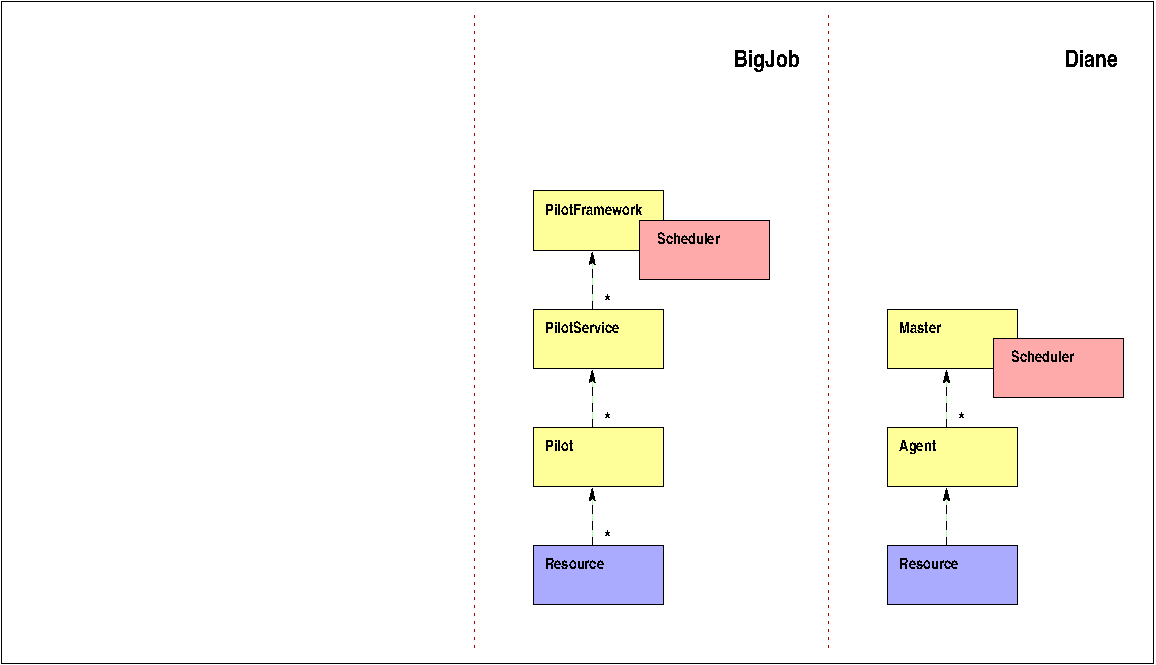
\includegraphics[height=5.5cm]{../architecture_overview_1.pdf}}
	  \only<2>{~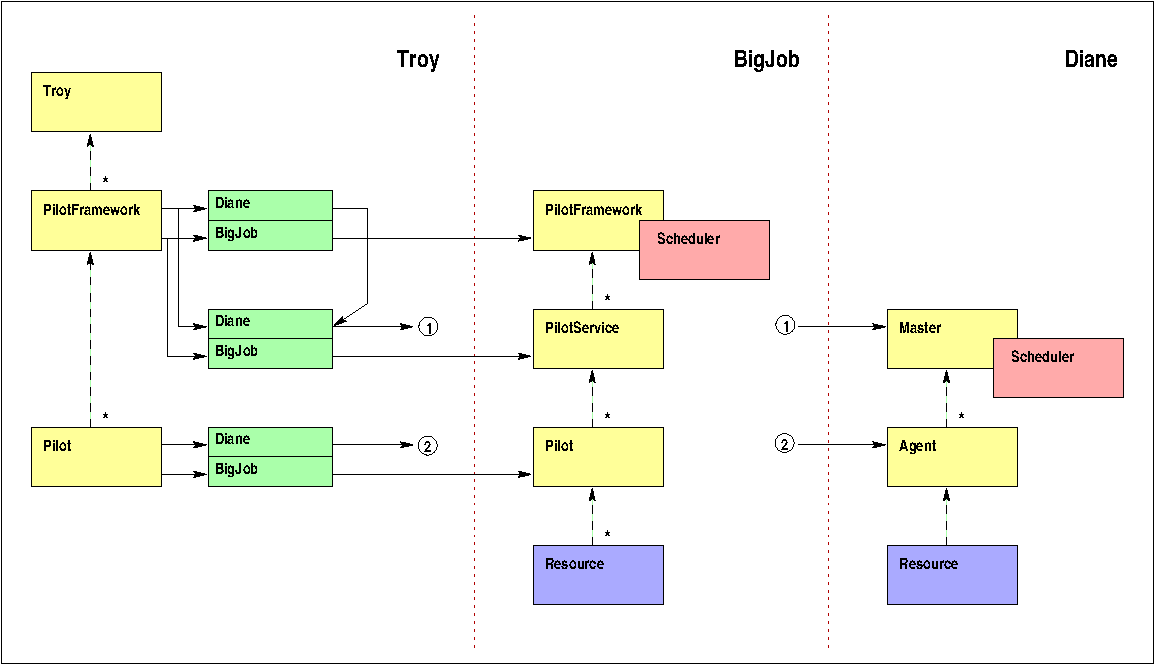
\includegraphics[height=5.5cm]{../architecture_overview_2.pdf}}
	  \only<3>{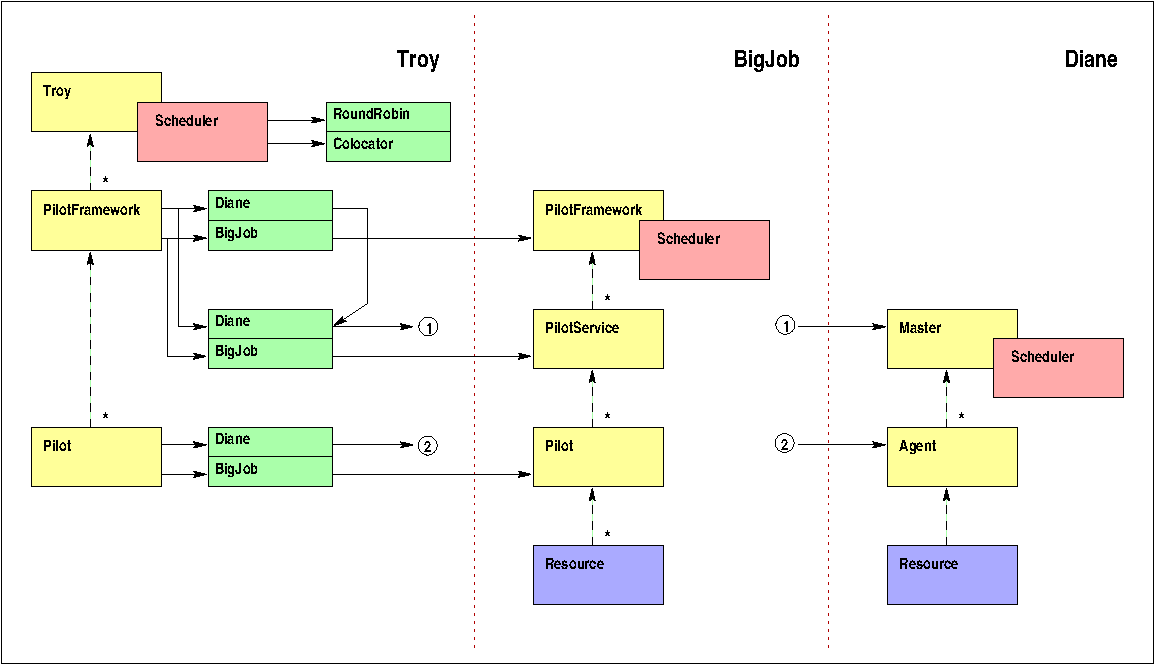
\includegraphics[height=5.5cm]{../architecture_overview_3.pdf}}
	  \only<4>{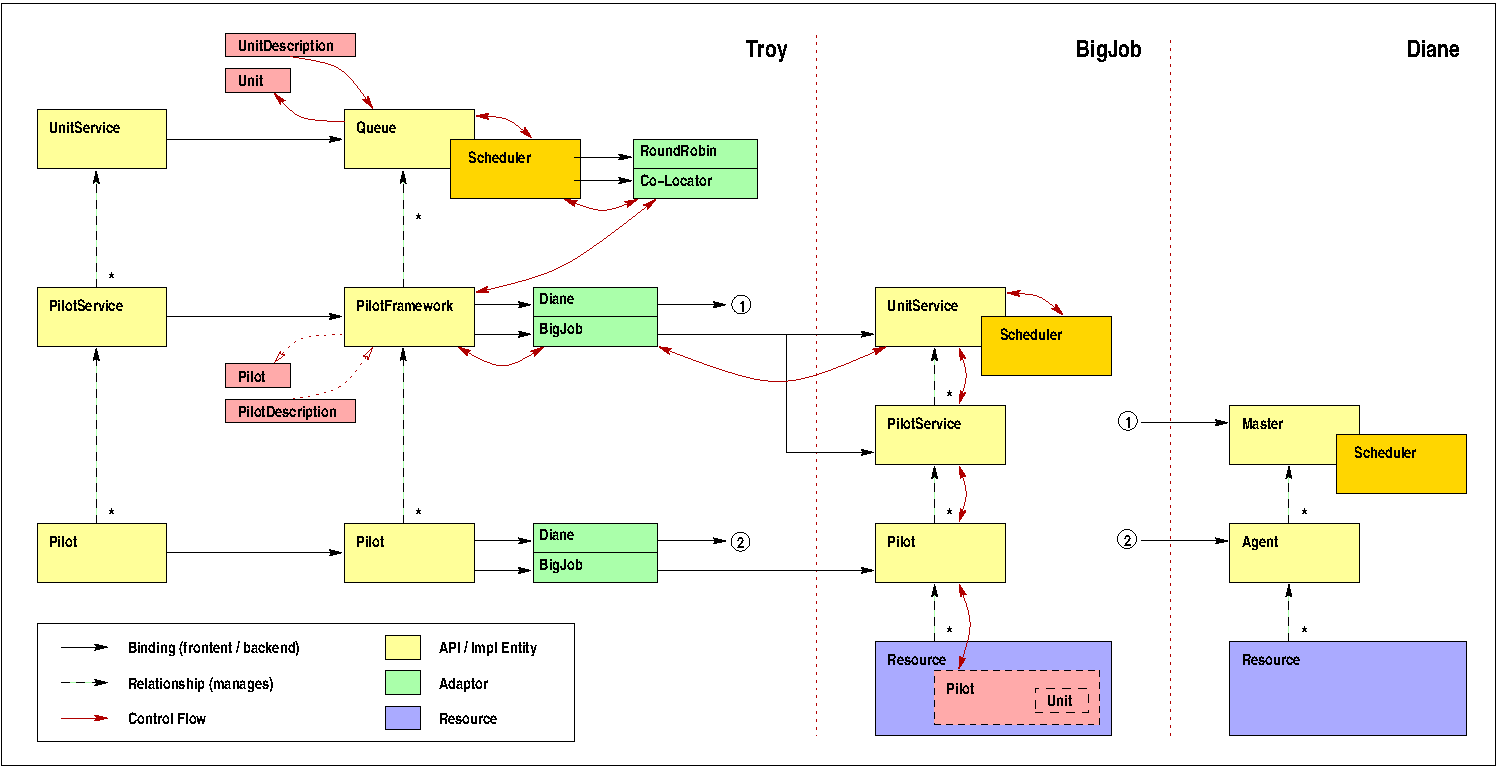
\includegraphics[height=5.5cm]{../architecture.pdf}}
	  \only<5>{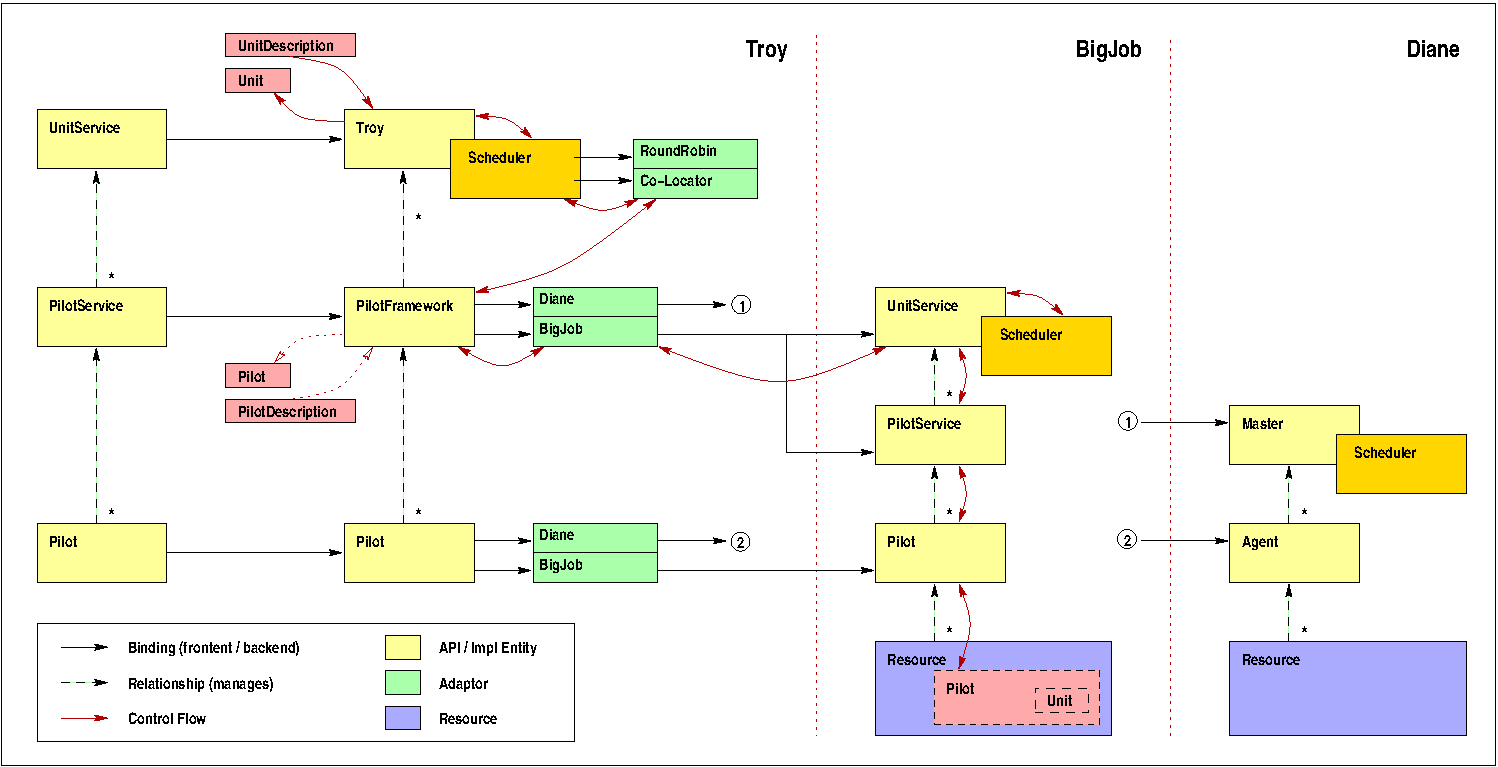
\includegraphics[height=5.5cm]{../architecture_pilot.pdf}}
  \end{center}
}

\section{Implementation Architecture / Design}

\begin{frame}[fragile]
	\frametitle{Troy API Classes}
   Troy classes interfacing to backend pilot systems:

  \begin{itemize}
    \item \verb|troy.Scheduler|\\
    \item \verb|troy.PilotFramework|\\
     interfaces to the \verb|XXXUnitService| and \verb|XXXPilotService|
     classes of Pilot API

    \item \verb|troy.ComputePilot|
    \item \verb|troy.ComputeUnit|

    \item \verb|troy.DataPilot|
    \item \verb|troy.DataUnit|
  \end{itemize}
\end{frame}

% \frame {
%   \frametitle{Scheduler}
% 
%   \verb|Scheduler| routines or adaptors need
%   information to make scheduling decisions:
% 
%   \begin{itemize}
%    \item inspect pilots (load, locality, type, ...)
%    \item inspect backend pilot system
%    \item inspect internal troy state (work items...)
%    \item out-of band system information (information services etc.)
%    \item application specific information sources
%    \item scheduler specific information sources
%   \end{itemize}
% }

\section{API, Code Example}

\begin{frame}[fragile] 
 \frametitle{Troy API}
 {\footnotesize
  \begin{block}{API Example}
   \begin{verbatim}
t   = troy.Troy ()
t.PilotFramework ('bigjob//lonestar')
t.PilotFramework ('bigjob//kraken')

s   = troy.Scheduler ('Random')
t.add_scheduler (s)

cpd  = troy.ComputePilotDescription ()
pf1.submit_pilot (cpd)
pf2.submit_pilot (cpd)
   \end{verbatim}
  \end{block}
 }
\end{frame}

\begin{frame}[fragile] 
 \frametitle{Troy API}
 {\footnotesize
  \begin{block}{API Example Cont.}
   \begin{verbatim}
cud  = troy.ComputeUnitDescription ()

cud['executable'] = '/bin/sh'
cud['arguments']  = ['-c', 'touch /tmp/hello_troy_pj && sleep 10']

cu  = t.submit_unit (cud)
   \end{verbatim}
  \end{block}
 }
\end{frame}

\begin{frame}[fragile] 
 \frametitle{Troy API}
 {\footnotesize
  \begin{block}{API Example Cont.}
   \begin{verbatim}
s_  = cu.state

while s_ != troy.State.Done and \
      s_ != troy.State.Failed   :

    print "cu : %s"  %  (str(s_))
    time.sleep (1)
    s_ = cu.state

print "cu : %s"  %  (str(s_))

cp1.cancel ()
cp2.cancel ()

pf.cancel ()
   \end{verbatim}
  \end{block}
 }
\end{frame}

\begin{frame}[fragile] 
 \frametitle{Troy API}
 {\footnotesize
  \begin{block}{Scheduler}
   \begin{verbatim}
def my_scheduler (troy, ud) :

    pf_ids = troy.list_pilot_frameworks ()
    pilots = []

    for pf_id in pf_ids :
        pf    = troy.PilotFramework (pf_id)
        p_ids = pf.list_pilots ()

        for p_id in p_ids :
            if _ud_is_compute (ud) :
                pilots.append (troy.ComputePilot (p_id))
            else :
                # ignore non-compute ud's
                pass
   \end{verbatim}
  \end{block}
 }
\end{frame}

\begin{frame}[fragile] 
 \frametitle{Troy API}
 {\footnotesize
  \begin{block}{Scheduler  Cont.}
   \begin{verbatim}
    idx = random.randint (0, len  (pilots) - 1)
    p   = pilots[idx]

    return p.submit_unit (ud)
   \end{verbatim}
  \end{block}
 }
\end{frame}



\begin{frame}[fragile] 
 \frametitle{Troy API}
 {\footnotesize
  \begin{block}{API Example + Scheduler}
   \begin{verbatim}
t   = troy.Troy ()
pf  = troy.PilotFramework ('bigjob//')
t.add_pilot_framework (pf)

s   = troy.Scheduler ('Random')
t.add_scheduler (s)

cpd  = troy.ComputePilotDescription ()
cp1  = pf.submit_pilot (cpd)
cp2  = pf.submit_pilot (cpd)
   \end{verbatim}
  \end{block}
 }
\end{frame}



% \begin{frame}[fragile] 
%  \frametitle{Troy API}
%  {\footnotesize
%    \begin{block}{API Example + Scheduler}
%     \code
%   \begin{Verbatim}
%  t   = troy.Troy ()
%  pf  = troy.PilotFramework ('bigjob//')
%  t.add_pilot_framework (pf)
%  
%  
%  t.add_scheduler (my_scheduler)
%  
%  cpd  = troy.ComputePilotDescription ()
%  cp1  = pf.submit_pilot (cpd)
%  cp2  = pf.submit_pilot (cpd)
%    \end{Verbatim}
%   \end{block}
%  }
% \end{frame}


\begin{frame}[fragile] 
 \frametitle{Troy API}
 {\footnotesize
   \begin{block}{API Example + Scheduler}
  \begin{verbatim}
t   = troy.Troy ()
pf  = troy.PilotFramework ('bigjob//')
t.add_pilot_framework (pf)


t.add_scheduler (my_scheduler)

cpd  = troy.ComputePilotDescription ()
cp1  = pf.submit_pilot (cpd)
cp2  = pf.submit_pilot (cpd)
   \end{verbatim}
  \end{block}
 }
\end{frame}



\end{document}

